\documentclass[titlepage]{article}
\usepackage[left=15mm,right=15mm,top=1in,bottom=1in]{geometry}
\usepackage{framed}
\usepackage{caption}
\usepackage{amsmath}
\usepackage{imakeidx}
\usepackage{graphicx}
\usepackage{array}
\usepackage{tikz}
\usetikzlibrary{automata,positioning,decorations.pathmorphing,shapes}

\newcolumntype{C}[1]{>{\centering\arraybackslash} m{#1cm}}

\makeindex

\title{Autonomous Pool Playing Robot\\~\\High-Level Architectural Design}
\author{
	Eric Le Fort\\leforte@mcmaster.ca\\1308609\\~\\\and
	Max Moore\\moorem8@mcmaster.ca\\1320009
}
 
\begin{document}
\maketitle
\tableofcontents
~\\[15mm]
\listoftables
\listoffigures


\vfill
\begin{table}[!htbp]
\centering
\begin{tabular}{| C{3} | C{2} | C{5} | C{2.5} |}\hline
	Date			&Revision \#	&Comments						&Authors\\\hline
	14/11/2016		&0				&- Initial document creation	&Eric Le Fort\newline Max Moore\\\hline
\end{tabular}
\caption{Revision History}
\end{table}
\newpage
 
\section{Introduction}
This document's purpose is to describe the architecture of the software controlling the Autonomous Pool Playing Robot. Both the architecture for the encompassing system as well as architectures for distinct subsystems will be discussed.
\subsection{System Description}
This system will provide a control system for an autonomous pool playing robot. It will include three separate computational units and four separate programs.\\~\\
The first computational unit will be a camera (likely a camera phone). This device will be responsible for reacting to a request, taking an image and then relaying that image.\\~\\
The next computational unit will be the PC. This device will have two separate programs that must execute for the system to be successful. One program will handle the VR and the other will handle shot selection as well as message passing between devices. The VR program will handle processing the image from the camera into a table state that can be used by the shot selection algorithm. The other program on the PC will handle performing an algorithm to determine which shot should be taken, where to move the cue in order to take that shot, instructing the camera to take pictures, receiving the image from the camera, receiving a signal to take a shot from the $\mu$C and communicating the shot that must be taken back to the $\mu$C.\\~\\
The last computational unit, the $\mu$C, will be responsible for interpreting the shot instructions provided by the PC into signals to control the machine accordingly, receiving control signals from the system, providing signals to move the machine out of the way to predetermined locations when requested, and sending the signal to take a shot back to the PC.
\subsection{Overview}
This document has four sections not including this one. Each section contains either design diagrams or further explanations to further describe the architecture of this system and is intended to prepare the software team to implement the design.\\
\begin{itemize}
	\item \textbf{Use Cases}: Describes possible user interactions with the system as well as the intended results of those interactions through the use of simple diagrams. A Use Case Diagram is also provided for reference.\\
	\item \textbf{Analysis Class Diagram}: Defines the various classes in the system, how they will be connected, and their type (boundary, controller, or entity).\\
	\item \textbf{Architectural Design}: This section defines the overall system architecture as well as the architectures of all subprograms.\\
	\item \textbf{CRC Cards}: Each program will be broken up into their specific classes. The responsibilities of each class as well as any collaboration required with other classes to fulfill each responsibility (if any) will be listed.\\
\end{itemize}

\subsection{Naming Conventions \& Definitions}
This section outlines the various definitions, acronyms and abbreviations that will be used throughout this document in order to familiarize the reader prior to reading.
\subsubsection{Definitions}
Table \ref{tab:Definitions} lists the definitions used in this document. The definitions given below are specific to this document and may not be identical to definitions of these terms in common use. The purpose of this section is to assist the user in understanding the requirements for the system.
\begin{table}[h!]
\centering
\caption{Definitions}
\begin{tabular}{| C{6} | p{6cm} |}\hline
	\textbf{Term}	&\textbf{\centering Meaning}\\\hline
	X-axis					&Distance along the length of the pool table\\\hline
	Y-axis					&Distance across the width of the pool table\\\hline
	Z-axis					&Height above the pool table\\\hline
	End-effector			&The end of the arm that will strike the cue ball\\\hline
	$\theta$				&Rotational angle of end-effector\\\hline
	Cue 					&End-effector\\\hline
	Personal Computer		&A laptop that will be used to run the more involved computational tasks such as visual recognition and the shot selection algorithm\\\hline
	Camera					&Some form of image capture device (e.g. a digital camera, smartphone with a camera, etc.)\\\hline
	Table State				&The current positions of all the balls on the table\\\hline
	Entity					&Classes that have a state, behaviour and identity (e.g. Book, Car, Person, etc.)\\\hline
	Boundary				&Classes that interact with users or external systems\\\hline
\end{tabular}
\label{tab:Definitions}
\end{table}

\newpage
\subsubsection{Acronyms \& Abbreviations}
Table \ref{tab:Acronyms} lists the acronyms and abbreviations used in this document.
\begin{table}[h!]
\centering
\caption{Acronyms and Abbreviations}
\begin{tabular}{| p{6cm} | p{6cm} |}\hline
	\textbf{Acronym/Abbreviation}	&\textbf{Meaning}\\\hline
	VR								&Visual Recognition\\\hline
	PC								&Personal Computer\\\hline
	$\mu$C							&Micro-Controller\\\hline
	CRC								&Class Responsibility Collaboration\\\hline
\end{tabular}
\label{tab:Acronyms}
\end{table}


\section{Use Cases}
This section will outline the use cases that this system will be expected to handle. A Use Case Diagram will also be provided to help illustrate these cases. All use cases are initiated by the user interacting with a physical interface that will send a signal to the $\mu$C. Between operations, the various programs will revert to a dormant state to await the next instruction.
\subsection{Use Case Diagram}%TODO include sensory calibration input into use-case diagram and use-cases?
The following diagram depicts the use cases of this system.\\
\begin{center}
	\includegraphics[width=\textwidth]{useCaseDiagram.png}
\captionof{figure}{Use Case Diagram}
\label{fig:use case diagram}
\end{center}
\subsection{Move Instruction}
This use case involves only the $\mu$C. The user presses the \textit{move} button. Once the signal has been received, the $\mu$C will decide which predetermined set point to move to based on the current position of the machine that is stored in its memory. The $\mu$C will then determine the signals required to relocate the machine to the appropriate location and then send them to the machine. Once those signals are sent, the $\mu$C will update its memory to store the new position of the machine.
\subsection{Cancel Instruction}
This use case involves only the $\mu$C. The user presses the \textit{cancel} button. Once the signal has been received, the $\mu$C will immediately stop the machine's motion. It will then update its memory to store the current position of the machine.
\subsection{Take a Shot Instruction}
This use case involves all four programs: the $\mu$C, the PC Controller Program, the Camera Program, and the PC VR Program in that order. The user presses the \textit{take a shot} button. Once the signal has been received, the $\mu$C will send a request to the PC to begin its process and wait a small amount of time for the PC to send a receipt response. If the $\mu$C does not receive a response within the specified timeframe, it will resend its request. This process will be repeated until a response is received. The PC Controller Program will then send a signal to the camera to take a photo. Upon receiving this signal, the camera will take a picture of the table and send this back to the PC. If the picture was received correctly, the PC Controller Program will then start the PC VR Program and provide the picture to be used. Otherwise, the PC Controller Program will continue to resend the request to take a picture as necessary. The PC VR Program will utilize object detection to determine where the balls are on the table and which ball is which. Once collecting this information, it is provided to the PC Controller Program through an intermediate file. The PC Controller Program will then use its shot selection algorithm to determine how to strike the pool ball to take based on the table state provided and transmit that shot to the $\mu$C. After that, the $\mu$C will send a receipt signal back to the PC Controller Program. The $\mu$C will interpret the shot information to create an instruction set of signals to move the machine appropriately and take the shot.
\subsection{Take a Shot Operation Interrupted During PC Computation}
This use case involves all four programs: the $\mu$C, the PC Controller Program, the Camera Program, and the PC VR Program in that order. The user presses the \textit{take a shot} button. Once the signal has been received, the $\mu$C will send a request to the PC to begin its process and wait a small amount of time for the PC to send a receipt response. If the $\mu$C does not receive a response within the specified timeframe, it will resend its request. This process will be repeated until a response is received. Sometime between this point and getting the selected shot communicated back to the $\mu$C, the user presses the \textit{cancel} button. The PC will complete its normal operation but once the shot is communicated back to the $\mu$C, it will simply be ignored.



\section{Analysis Class Diagrams}
%TODO create these diagrams in draw.io
\subsection{$\mu$C Analysis Class Diagram}
%TODO
\subsection{PC Controller Analysis Class Diagram}
%TODO
\subsection{Camera Analysis Class Diagram}
%TODO 
\subsection{PC VR Program Analysis Class Diagram}
%TODO



\section{Architectural Design}
This section will discuss the architectures that are to be used while designing this system. The goal of these architectures is to promote the overall quality of the software for this system. In particular, the software should be more efficient, robust, and maintainable as a result of this architectural design.
\subsection{System Architecture}
The architecture of this system as a whole will be modelled using the \textit{Batch Sequential} style. This architecture involves sending chunks of data after each program is completely done processing and promotes simple division of subsystems that can operate as independent programs. This creates a strong separation of concerns within the larger system.\\~\\
The shortcomings of this system are that it does not allow for concurrency and it has low throughput. Luckily, in this situation, the throughput is not intended to be very high. Also, each subsystem must wait for the previous system to fully complete its task in order to proceed regardless. Therefore, since this system does not even allow for concurrent operation, there is no loss in potential efficiency.
\subsection{Subsystems}
The subsystems will follow the batch sequential architecture on a system level but that architecture does not make sense for the subsystems themselves. This section will discuss the architectures that will be utilized on the subsystem level.
\subsubsection{$\mu$C Architecture}
This subsystem will utilize a \textit{Sensor-Controller-Actuator} architecture style. This style is well-suited to embedded systems that deal with hardware which is optimal for this subsystem. The style breaks the subsystem up into four types of components: interfaces, sensors, actuators, and a controller. An illustration of the architecture is provided below:\\
\begin{center}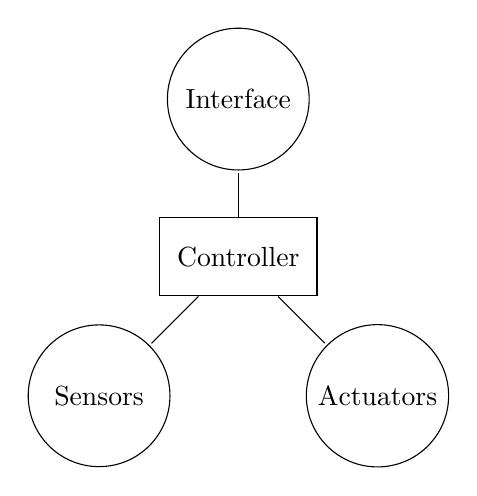
\begin{tikzpicture}[shorten >=1pt,on grid,auto]
	\node[rectangle, draw, scale=1, minimum width=2cm,minimum height=1cm](0) []{Controller};
	\node[circle, draw,node distance=2.0cm, minimum size=1.8cm](1) [above of=0]{Interface};
   	\node[circle, draw,node distance=2.5cm, minimum size=1.8cm](2) [below left of=0]{Sensors};
	\node[circle, draw,node distance=2.5cm, minimum size=1.8cm](3) [below right of=0]{Actuators};
   	\draw (0) -- (1);
	\draw (0) -- (2);
	\draw (0) -- (3);
\end{tikzpicture}
\captionof{figure}{Sensor-Controller-Actuator Architecture}
\label{fig:Sensor-Controller-Actuator Architecture}
\end{center}~\\
In the case of this subsystem, the breakdown of the components into these types will be as follows:
\begin{itemize}
	\item Sensors - System State
	\begin{itemize}
		\item Calibration sensors (quantity yet to be determined)
	\end{itemize}
	\item Sensors - Interface
	\begin{itemize}
		\item Stop buttons (multiple located throughout machine, quantity yet to be determined)
		\item Move button
		\item Take shot button
	\end{itemize}
	\item Logic
	\begin{itemize}
		\item Motion logic
		\item Current state info
	\end{itemize}
	\item Actuators
	\begin{itemize}
		\item Translational motors ($\times2$)
		\item Rotational motor
		\item Pneumatic end-effector
	\end{itemize}
\end{itemize}
\subsubsection{PC Controller Architecture}
This subsystem will utilize a \textit{Rule-Based} architecture style. This style is well suited to making strategic moves while playing a game with rigid rules constraining actions. In other words, for deciding which shot is the best to take given the current state of table and the rules of the game of pool. This style breaks down the subsystem into four types of modules: an interface, a rule-set,  working memory, and an inference engine. The interface will be where the system gets its input and sends its output. The rule-set is a particular sort of knowledge base that contains the rules constraining the acceptable actions. The working memory is temporary memory used by the subsystem. Lastly, the inference engine is what ties the subsystem together. Its job is to apply the rules appropriately and, using the working memory as a tool, generate the appropriate result to send as output.\\~\\
In the case of this subsystem, the breakdown of these modules into these types will be as follows:
\begin{itemize}
	\item Interface
	\begin{itemize}
		\item Input -- table state
		\item Output -- specification of shot (position, angle, and force)
	\end{itemize}
	\item Rule-Set
	\begin{itemize}
		\item Rules of pool
		\item Mechanical constraints
		\item Physical constants (i.e. ball weight, table friction, spring constant of table cushions, etc.)
	\end{itemize}
	\item Working Memory
	\begin{itemize}
		\item Table state
		\item Current optimal shot
	\end{itemize}
	\item Inference Engine
	\begin{itemize}
		\item Simulate results of shots
		\item Check rules against shot simulations at some incremental angle
		\item Score shots based on weighted application of rules
	\end{itemize}
\end{itemize}
\subsubsection{Camera Architecture}
This subsystem will utilize an \textit{Event-Driven} architectural style. This will likely be the simplest subsystem present in the system. The role of this program is to sit idle waiting for a request to take a picture. Once it receives that request, it should take a picture and then communicate that image back to the PC Controller program. This request is the only event this program must respond to.
\subsubsection{PC VR Program Architecture}
This subsystem will also utilize a \textit{Batch Sequential} architecture style. This style has already been discussed in the system architecture and so will not be discussed again here. In this subsystem, the process is begun upon receipt of the request to start operation. The subsystem will then utilize a MATLAB VR library to detect the balls as objects on the table using the image provided. The results of this will be passed to the next step which will use the positions of the identified objects to determine which specific ball is which using colour comparison. Once this step completes, the table state has been computed and is then sent back to the PC Controller program. The issues of low throughput and lack of concurrency are not an issue in this case as the system would have to wait for the previous step to complete in order to begin the next step anyway.\\~\\

An illustration of the specific implementation of this architecture is provided below:\\~\\
$$\text{in } \xrightarrow{\text{image}} \text{ object detection } \overset{\text{image \&}}{\xrightarrow{\text{object positions}}} \text{ ball identification } \xrightarrow{\text{table state}} \text{ out}$$
\captionof{figure}{PC VR Architecture}
\label{fig:PC VR Architecture}



\section{Class Responsibility Collaboration (CRC) Cards}
This section provides CRC cards for all classes in each of the programs. Each card will list the responsibilities as well as any classes the must be collaborated with to perform that responsibility.
\subsection{$\mu$C CRC Cards}
The following are the CRC cards for the $\mu$C program:\\
%TODO

\subsection{PC Controller CRC Cards}
The following are the CRC cards for the PC Controller program:\\
\begin{table}[!htbp]%TODO collaborators
\centering
\begin{tabular}{| p{0.5\textwidth} | p{0.3\textwidth} |}\hline
	\multicolumn{2}{|l|}{}\\
	\multicolumn{2}{|c|}{\large{\textbf{Communicator}}}\\
	\multicolumn{2}{|l|}{}\\\hline
	\vspace{0mm}\large{Responsibilities}\vspace{2mm} &\vspace{0mm}\large{Collaborators}\vspace{2mm}\\\hline
	\vspace{0mm}- Listens for request from $\mu$C	&\vspace{0mm}-\\&\\
	- Sends confirmation of receipt to $\mu$C		&-\\&\\
	- Sends shot specification to $\mu$C			&-\\&\\
	- Listen for receipt confirmation from $\mu$C	&-\\&\\
	- Sends image capture request to camera			&EventHandler\\&\\
	- Listens for response from camera				&EventHandler\\&\\
	- Initiate the PC VR program					&(None)\\&\\
	- Read table state from file\vspace{2mm}		&(None)\vspace{2mm}\\\hline
\end{tabular}
\end{table}

\begin{table}[!htbp]
\centering
\begin{tabular}{| p{0.5\textwidth} | p{0.3\textwidth} |}\hline
	\multicolumn{2}{|l|}{}\\
	\multicolumn{2}{|c|}{\large{\textbf{Vector}}}\\
	\multicolumn{2}{|l|}{}\\\hline
	\vspace{0mm}\large{Responsibilities}\vspace{2mm} &\vspace{0mm}\large{Collaborators}\vspace{2mm}\\\hline
	\vspace{0mm}- Stores and allows access to an x- and y-component of a vector	&\vspace{0mm}(None)\\\hline
\end{tabular}
\end{table}

\begin{table}[!htbp]
\centering
\begin{tabular}{| p{0.5\textwidth} | p{0.3\textwidth} |}\hline
	\multicolumn{2}{|l|}{}\\
	\multicolumn{2}{|c|}{\large{\textbf{Ball}}}\\
	\multicolumn{2}{|l|}{}\\\hline
	\vspace{0mm}\large{Responsibilities}\vspace{2mm} &\vspace{0mm}\large{Collaborators}\vspace{2mm}\\\hline
	\vspace{0mm}- Store and allow access to its position							&\vspace{0mm}Vector\\&\\
	- Store and allow access to the value representing its identity\vspace{2mm}		&(None)\vspace{2mm}\\\hline
\end{tabular}
\end{table}

\begin{table}[!htbp]
\centering
\begin{tabular}{| p{0.5\textwidth} | p{0.3\textwidth} |}\hline
	\multicolumn{2}{|l|}{}\\
	\multicolumn{2}{|c|}{\large{\textbf{Shot}}}\\
	\multicolumn{2}{|l|}{}\\\hline
	\vspace{0mm}\large{Responsibilities}\vspace{2mm} &\vspace{0mm}\large{Collaborators}\vspace{2mm}\\\hline
	\vspace{0mm}- Store and allow access to the position from which to take this shot	&\vspace{0mm}Vector\\&\\
	- Store and allow access to the angle from which to take this shot					&(None)\\&\\
	- Store and allow access to the amount of power to use to take this shot			&(None)\\&\\
	- Store and allow access to the scoring assigned to this shot\vspace{2mm}			&(None)\vspace{2mm}\\\hline
\end{tabular}
\end{table}

\begin{table}[!htbp]
\centering
\begin{tabular}{| p{0.5\textwidth} | p{0.3\textwidth} |}\hline
	\multicolumn{2}{|l|}{}\\
	\multicolumn{2}{|c|}{\large{\textbf{TableState}}}\\
	\multicolumn{2}{|l|}{}\\\hline
	\vspace{0mm}\large{Responsibilities}\vspace{2mm} &\vspace{0mm}\large{Collaborators}\vspace{2mm}\\\hline
	\vspace{0mm}- Store and allow access to the positions of the balls present on the table		&\vspace{0mm}Ball, Vector\\&\\
	- Store and allow access to the number of both types of ball on the table\vspace{2mm}		&Ball\vspace{2mm}\\\hline
\end{tabular}
\end{table}

\begin{table}[!htbp]
\centering
\begin{tabular}{| p{0.5\textwidth} | p{0.3\textwidth} |}\hline
	\multicolumn{2}{|l|}{}\\
	\multicolumn{2}{|c|}{\large{\textbf{TableStateSimulationInstance}}}\\
	\multicolumn{2}{|l|}{}\\\hline
	\vspace{0mm}\large{Responsibilities}\vspace{2mm} &\vspace{0mm}\large{Collaborators}\vspace{2mm}\\\hline
	\vspace{0mm}- Maintain the positions and velocities of balls on the table at the current time step	&\vspace{0mm}TableState, Vector\\&\\
	- Update the positions and velocities of balls after one time step									&TableState, Vector\\&\\
	- Keep track of whether there is still movement occurring											&Vector\\&\\
	- Keep track of the scoring of the simulation (of a shot)\vspace{2mm}								&TableState\vspace{2mm}\\\hline
\end{tabular}
\end{table}

\begin{table}[!htbp]
\centering
\begin{tabular}{| p{0.5\textwidth} | p{0.3\textwidth} |}\hline
	\multicolumn{2}{|l|}{}\\
	\multicolumn{2}{|c|}{\large{\textbf{InferenceEngine}}}\\
	\multicolumn{2}{|l|}{}\\\hline
	\vspace{0mm}\large{Responsibilities}\vspace{2mm} &\vspace{0mm}\large{Collaborators}\vspace{2mm}\\\hline
	\vspace{0mm}- Calculate the shot to be made		&\vspace{0mm} TableStateSimulationInstance,\newline TableState, Shot, Vector\\&\\\hline
\end{tabular}
\end{table}

\subsection{Camera CRC Cards}
The following is the CRC card for the Camera program:\\
\begin{table}[!htbp]
\centering
\begin{tabular}{| p{0.5\textwidth} | p{0.3\textwidth} |}\hline
	\multicolumn{2}{|l|}{}\\
	\multicolumn{2}{|c|}{\large{\textbf{Event Handler}}}\\
	\multicolumn{2}{|l|}{}\\\hline
	\vspace{0mm}\large{Responsibilities}\vspace{2mm} &\vspace{0mm}\large{Collaborators}\vspace{2mm}\\\hline
	\vspace{0mm}- Listen for request from PC Controller	&\vspace{0mm}Communicator\\&\\
	- Take a photo										&(None)\\&\\
	- Communicate the photo\vspace{2mm}					&Communicator\vspace{2mm}\\\hline
\end{tabular}
\end{table}

\subsection{PC VR Program CRC Cards}
The following is the CRC card for the PC VR program:\\
\begin{table}[!htbp]
\centering
\begin{tabular}{| p{0.5\textwidth} | p{0.3\textwidth} |}\hline
	\multicolumn{2}{|l|}{}\\
	\multicolumn{2}{|c|}{\large{\textbf{TableStateVR}}}\\
	\multicolumn{2}{|l|}{}\\\hline
	\vspace{0mm}\large{Responsibilities}\vspace{2mm} &\vspace{0mm}\large{Collaborators}\vspace{2mm}\\\hline
	\vspace{0mm}- Read image from a file		&\vspace{0mm}(None)\\&\\
	- Locate balls using VR						&(None)\\&\\
	- Determine ball identities					&(None)\\&\\
	- Write table state to a file\vspace{2mm}	&(None)\vspace{2mm}\\\hline
\end{tabular}
\end{table}



\pagebreak
\printindex
\end{document}

\begin{table}[!htbp]
\centering
\begin{tabular}{| p{0.5\textwidth} | p{0.3\textwidth} |}\hline
	\multicolumn{2}{|l|}{}\\
	\multicolumn{2}{|c|}{\large{\textbf{CLASS\_NAME}}}\\
	\multicolumn{2}{|l|}{}\\\hline
	\vspace{0mm}\large{Responsibilities}\vspace{2mm} &\vspace{0mm}\large{Collaborators}\vspace{2mm}\\\hline
	\vspace{0mm}-	&\vspace{0mm}-\\&\\
	-				&-\\&\\
	-\vspace{2mm}	&-\vspace{2mm}\\\hline
\end{tabular}
\end{table}

